\documentclass[dvisvgm,tikz]{standalone}
\begin{document}
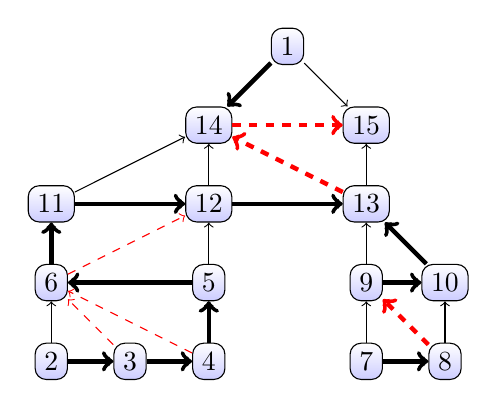
\begin{tikzpicture}

\node[shape=rectangle, rounded corners, draw, align=center, top color=white, bottom color=blue!20] (n1) at (3.0,4.0) {1};
\node[shape=rectangle, rounded corners, draw, align=center, top color=white, bottom color=blue!20] (n2) at (0.0,0.0) {2};
\node[shape=rectangle, rounded corners, draw, align=center, top color=white, bottom color=blue!20] (n3) at (1.0,0.0) {3};
\node[shape=rectangle, rounded corners, draw, align=center, top color=white, bottom color=blue!20] (n4) at (2.0,0.0) {4};
\node[shape=rectangle, rounded corners, draw, align=center, top color=white, bottom color=blue!20] (n5) at (2.0,1.0) {5};
\node[shape=rectangle, rounded corners, draw, align=center, top color=white, bottom color=blue!20] (n6) at (0.0,1.0) {6};
\node[shape=rectangle, rounded corners, draw, align=center, top color=white, bottom color=blue!20] (n7) at (4.0,0.0) {7};
\node[shape=rectangle, rounded corners, draw, align=center, top color=white, bottom color=blue!20] (n8) at (5.0,0.0) {8};
\node[shape=rectangle, rounded corners, draw, align=center, top color=white, bottom color=blue!20] (n9) at (4.0,1.0) {9};
\node[shape=rectangle, rounded corners, draw, align=center, top color=white, bottom color=blue!20] (n10) at (5.0,1.0) {10};
\node[shape=rectangle, rounded corners, draw, align=center, top color=white, bottom color=blue!20] (n11) at (0.0,2.0) {11};
\node[shape=rectangle, rounded corners, draw, align=center, top color=white, bottom color=blue!20] (n12) at (2.0,2.0) {12};
\node[shape=rectangle, rounded corners, draw, align=center, top color=white, bottom color=blue!20] (n13) at (4.0,2.0) {13};
\node[shape=rectangle, rounded corners, draw, align=center, top color=white, bottom color=blue!20] (n14) at (2.0,3.0) {14};
\node[shape=rectangle, rounded corners, draw, align=center, top color=white, bottom color=blue!20] (n15) at (4.0,3.0) {15};
\draw[->] (n1) -- (n14);
\draw[->] (n1) -- (n15);
\draw[->] (n2) -- (n3);
\draw[->] (n2) -- (n6);
\draw[->] (n3) -- (n4);
\draw[->] (n4) -- (n5);
\draw[->] (n5) -- (n6);
\draw[->] (n5) -- (n12);
\draw[->] (n6) -- (n11);
\draw[->] (n7) -- (n8);
\draw[->] (n7) -- (n9);
\draw[->] (n8) -- (n10);
\draw[->] (n9) -- (n10);
\draw[->] (n9) -- (n13);
\draw[->] (n10) -- (n13);
\draw[->] (n11) -- (n12);
\draw[->] (n11) -- (n14);
\draw[->] (n12) -- (n13);
\draw[->] (n12) -- (n14);
\draw[->] (n13) -- (n15);
\draw[red,dashed,->] (n3) -- (n6);
\draw[red,dashed,->] (n4) -- (n6);
\draw[red,dashed,->] (n6) -- (n12);
\draw[red,dashed,->] (n8) -- (n9);
\draw[red,dashed,->] (n13) -- (n14);
\draw[red,dashed,->] (n14) -- (n15);
\draw[ultra thick,->] (n1) -- (n14);
\draw[ultra thick,->] (n2) -- (n3);
\draw[ultra thick,->] (n3) -- (n4);
\draw[ultra thick,->] (n4) -- (n5);
\draw[ultra thick,->] (n5) -- (n6);
\draw[ultra thick,->] (n6) -- (n11);
\draw[ultra thick,->] (n7) -- (n8);
\draw[ultra thick,red,dashed,->] (n8) -- (n9);
\draw[ultra thick,->] (n9) -- (n10);
\draw[ultra thick,->] (n10) -- (n13);
\draw[ultra thick,->] (n11) -- (n12);
\draw[ultra thick,->] (n12) -- (n13);
\draw[ultra thick,red,dashed,->] (n13) -- (n14);
\draw[ultra thick,red,dashed,->] (n14) -- (n15);
\end{tikzpicture}
\end{document}

